\newpage

\section{Introduction}
\subsection{Shughni}
\par The Shughni language (ISO: sgh; glottolog: shug1248) is a low-resource language. It belongs to the Iranian branch of the Indo-European family \parencite[12]{plungian_study_2022}, and it is spoken by circa 80 000--100 000 people \parencite{edelman_dodykhudoeva_shughni_2009} on the territories of regions of Tajikistan and Afghanistan. Both regions have a subregion, where Shughni language is the most spoken native language, the subregions are called `Shughnon' in Tajikistan and `Shughnan' in Afghanistan \parencite[2]{parker_shughni_2023}, see Figure \ref{fig:map1} for details. Shughni is one of `Pamiri' languages, which is an areal group of languages spoken in the Pamir Mountains, primarily along the Panj river. Shughni has a mixed morphological typology type \parencite[94]{parker_shughni_2023}, which means that grammatical meanings can be carried by morphemes, words and clitics. There are three scripts for Shughni language: Latin, Cyrillic and Arabic. The Arabic script is used on the territory of Badakhshan Province of Afghanistan, and Cyrillic and Latin scripts are used in the Mountainous Badakhshan Autonomous Region of Tajikistan. The Latin script was created and gained popularity in 1930s, after it was set as the primary script for teaching in schools on the Shughni-speaking territory of Tajikistan. Later in 1980s a Cyrillic script was created \parencite[788]{edelman_dodykhudoeva_shughni_2009}.
\begin{figure}[h]
    \centering
    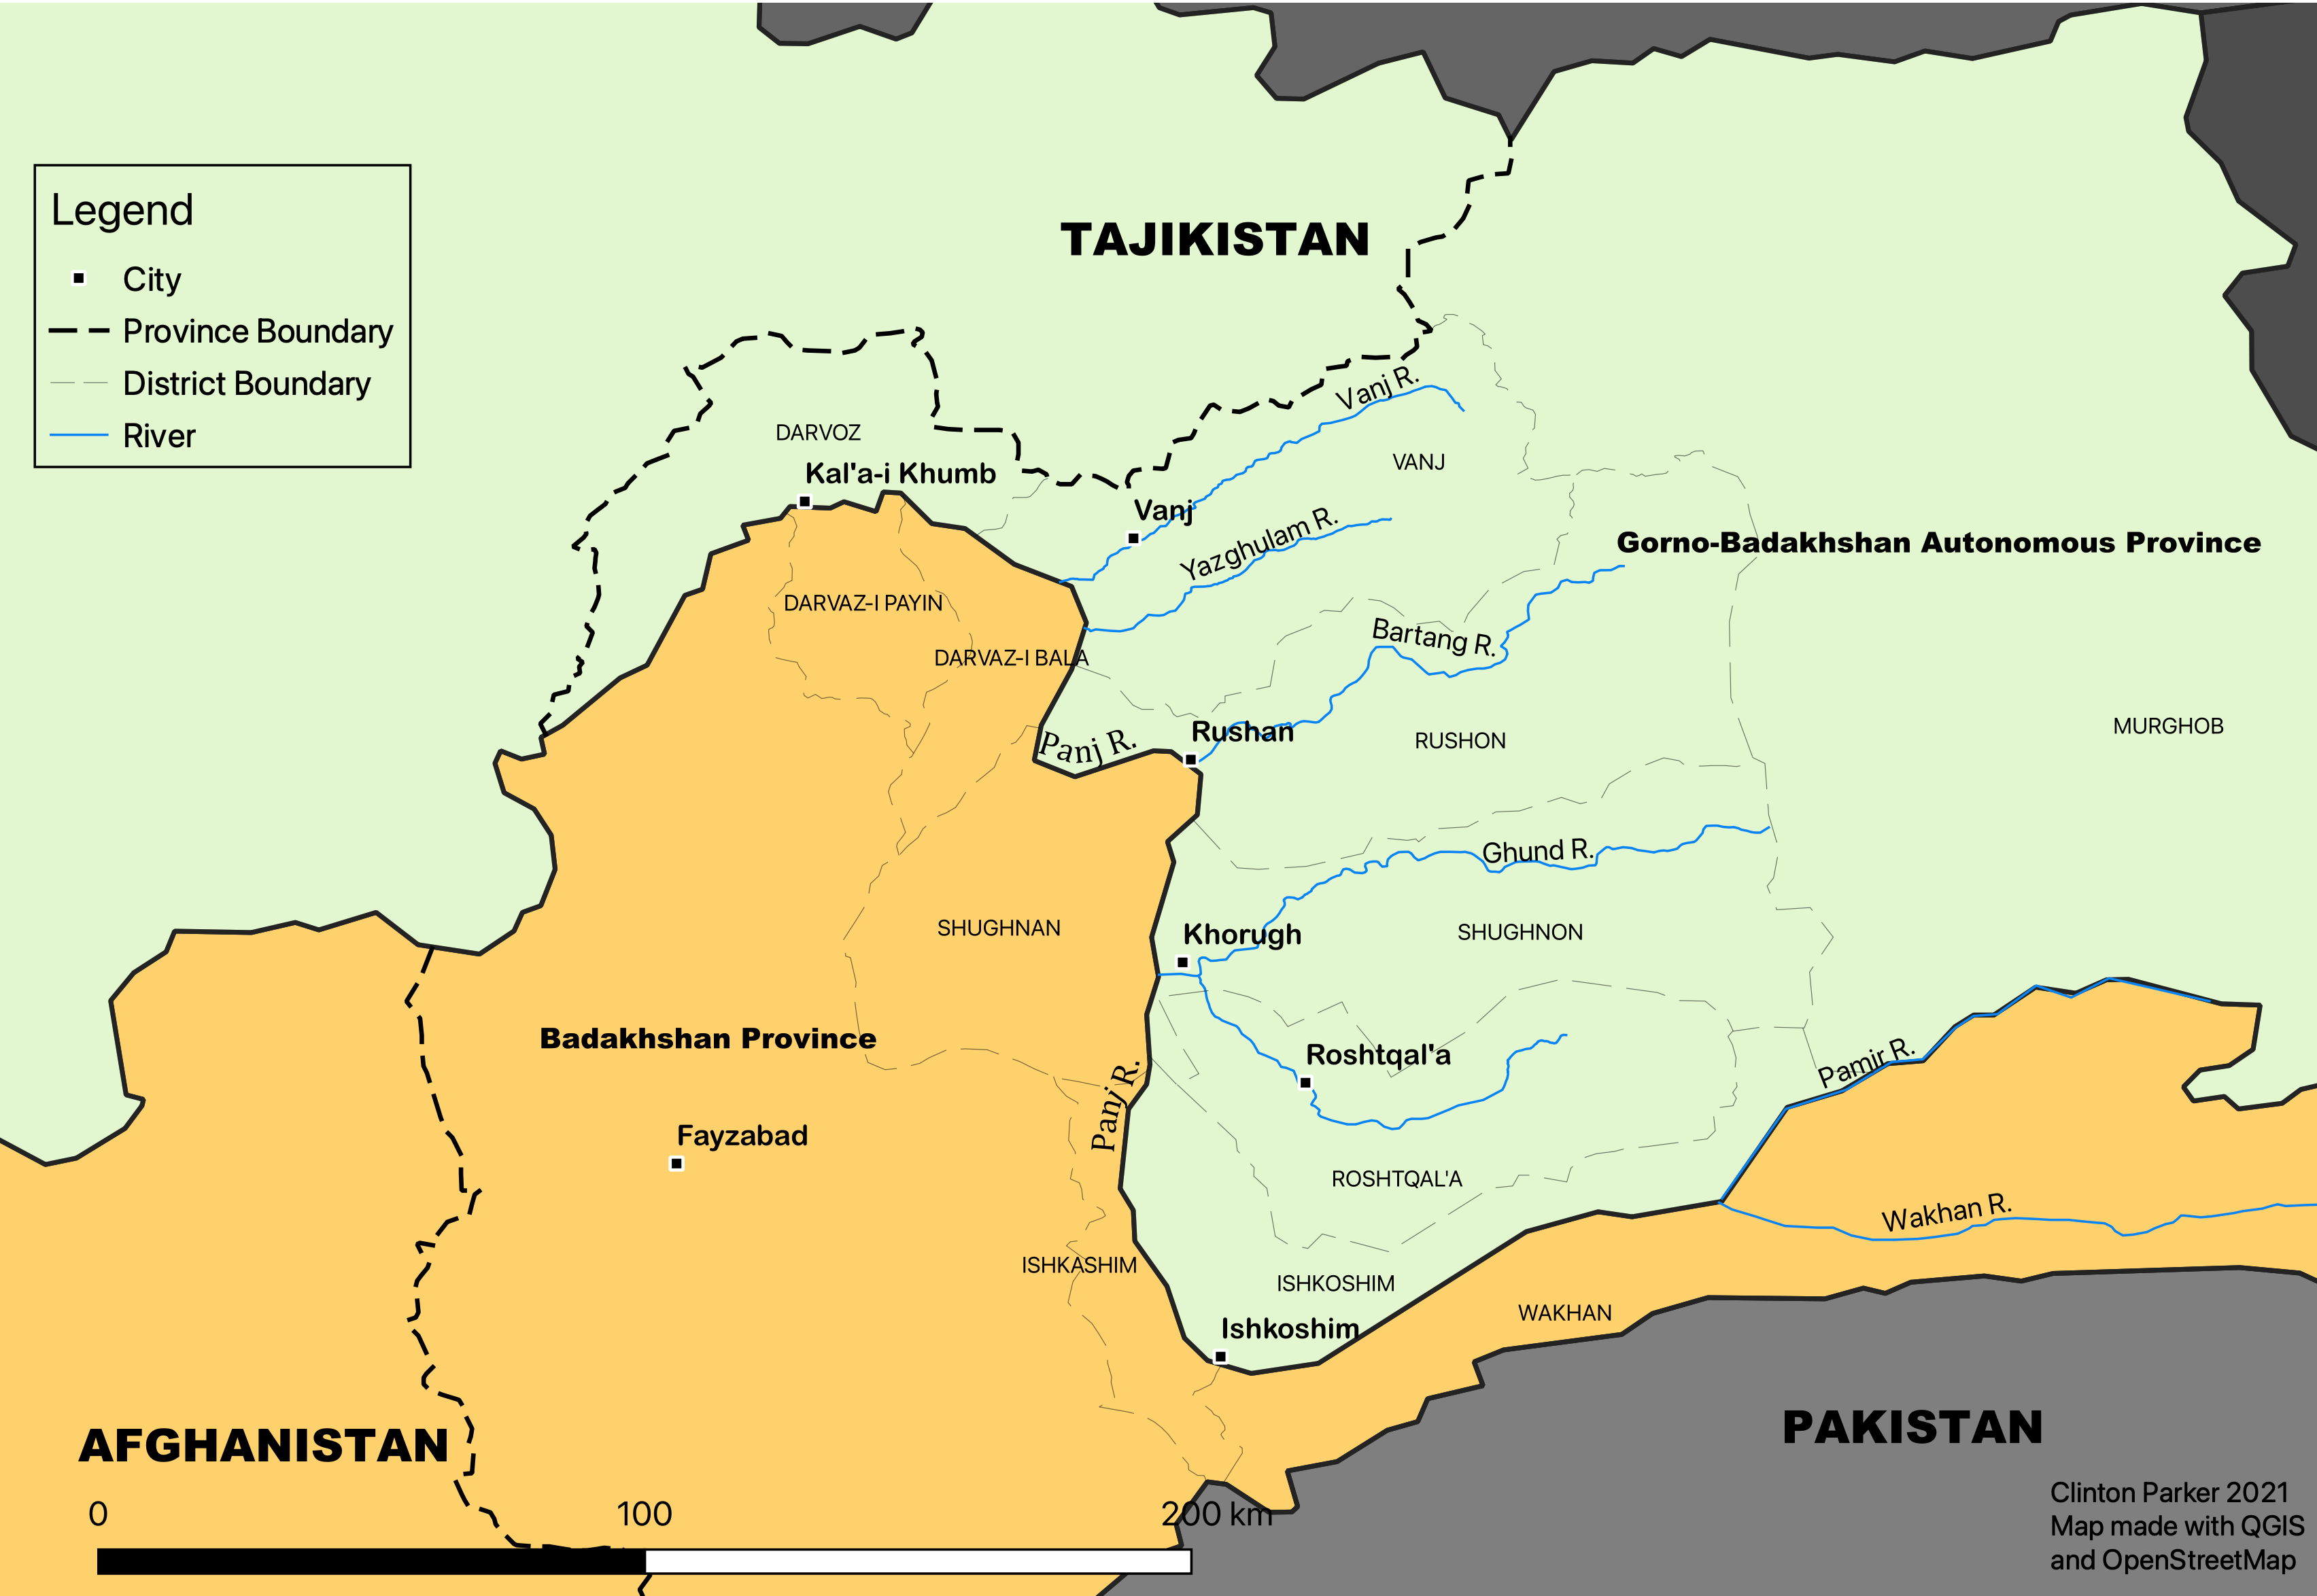
\includegraphics[scale=0.125]{\rootdir/img/map.png}
    \caption{Mountainous Badakhshan Autonomous Province of Tajikistan and Badakhshan Province of Afghanistan, \parencite[Fig 1.1]{parker_shughni_2023}}
    \label{fig:map1}
\end{figure}
\par Morphology analysis tools in question will focus on the variation of Shughni that is spoken in Tajikistan. Cyrillic and Latin script will be supported: the core analysis tool will be implemented in Cyrillic script, and Latin script support will be implemented via transliteration. Clitics will be relevant to this work, since in target Cyrillic and Latin scripts they often attach to words either with a hyphen or through direct affixation and therefore enter the scope of morphology.

\subsection{Morphology parsing}
\par Morphological parser is a fundamental tool, a wide range of computational linguistics' tasks such as POS-tagging, lemmatization and machine translation rely on some form of morphological model. For morphologically rich languages it is close to impossible to list and manually define all the possible word-forms. An alternative solution is to model the language's morphology instead.
\par For high-resource languages morphology modeling today is usually approached using deep learning (DL) models such as BERT \parencite{devlin-etal-2019-bert}, which are trained on large amounts of data. This method is not always available for low-resource languages that lack digital textual data, for such languages linguists apply rule-based approach.
\par Shughni is a low-resource language with very few data available, which leaves us the rule-based option. In this work Helsinki Finite-State Technology (HFST) will be used, which is a tool set that allows creating and manipulating finite-state transducers (FSTs). As it will be described below, FSTs can be used to model natural language's morphology and create morphological parsers. Modeling Shughni morphology using FST should not bring challenges. Its morphology is mostly agglunative and there are very few morphonological rules, the biggest challenge seems to be presented by clitics, which attach to words becoming part of morphology and which may carry information that exceeds the scope of morphology. Nouns, numerals, pronouns and preposition were implemented into a HFST morphological parser in my previous work \parencite{osorgin_2024_twol}. This work will fill the crucial gaps: verbs and adjectives.